\documentclass{minimal}
\usepackage{bm}
\usepackage{epsfig,color}
\usepackage[papersize={576.00bp,432.00bp},text={576.00bp,432.00bp}]{geometry}
\begin{document}
\centering
% Title: glps_renderer figure
% Creator: GL2PS 1.3.8, (C) 1999-2012 C. Geuzaine
% For: Octave
% CreationDate: Wed Jul 29 11:40:10 2015
\setlength{\unitlength}{1pt}
\begin{picture}(0,0)
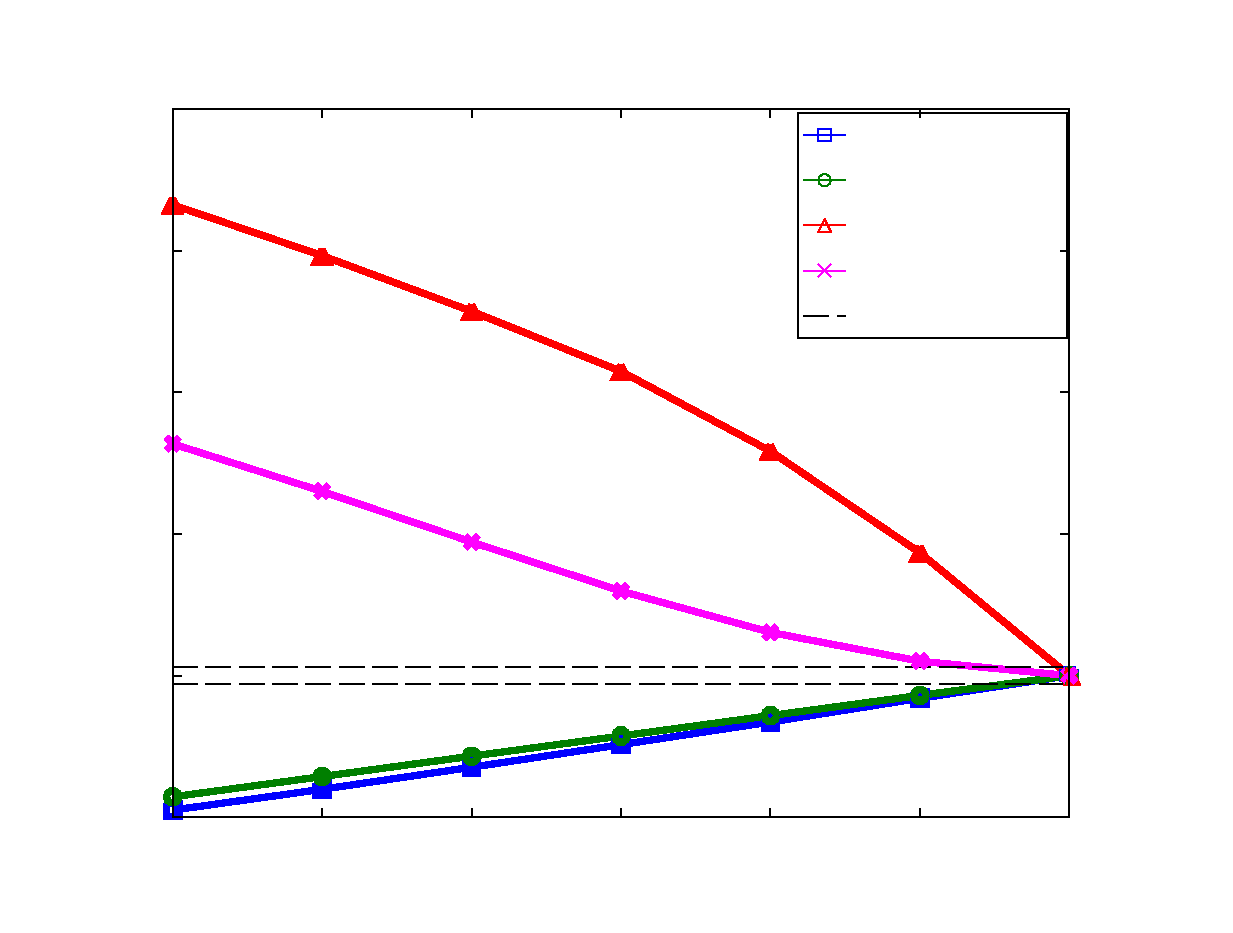
\includegraphics{fig_c1p-inc}
\end{picture}%
\begin{picture}(576,432)(0,0)
\fontsize{16}{0}
\selectfont\put(74.88,42.5188){\makebox(0,0)[t]{\textcolor[rgb]{0,0,0}{{1}}}}
\fontsize{16}{0}
\selectfont\put(146.613,42.5188){\makebox(0,0)[t]{\textcolor[rgb]{0,0,0}{{2}}}}
\fontsize{16}{0}
\selectfont\put(218.347,42.5188){\makebox(0,0)[t]{\textcolor[rgb]{0,0,0}{{3}}}}
\fontsize{16}{0}
\selectfont\put(290.08,42.5188){\makebox(0,0)[t]{\textcolor[rgb]{0,0,0}{{4}}}}
\fontsize{16}{0}
\selectfont\put(361.813,42.5188){\makebox(0,0)[t]{\textcolor[rgb]{0,0,0}{{5}}}}
\fontsize{16}{0}
\selectfont\put(433.547,42.5188){\makebox(0,0)[t]{\textcolor[rgb]{0,0,0}{{6}}}}
\fontsize{16}{0}
\selectfont\put(505.28,42.5188){\makebox(0,0)[t]{\textcolor[rgb]{0,0,0}{{7}}}}
\fontsize{16}{0}
\selectfont\put(69.8753,47.52){\makebox(0,0)[r]{\textcolor[rgb]{0,0,0}{{-10}}}}
\fontsize{16}{0}
\selectfont\put(69.8753,115.536){\makebox(0,0)[r]{\textcolor[rgb]{0,0,0}{{0}}}}
\fontsize{16}{0}
\selectfont\put(69.8753,183.552){\makebox(0,0)[r]{\textcolor[rgb]{0,0,0}{{10}}}}
\fontsize{16}{0}
\selectfont\put(69.8753,251.568){\makebox(0,0)[r]{\textcolor[rgb]{0,0,0}{{20}}}}
\fontsize{16}{0}
\selectfont\put(69.8753,319.584){\makebox(0,0)[r]{\textcolor[rgb]{0,0,0}{{30}}}}
\fontsize{16}{0}
\selectfont\put(69.8753,387.6){\makebox(0,0)[r]{\textcolor[rgb]{0,0,0}{{40}}}}
\fontsize{16}{0}
\selectfont\put(290.08,29.5188){\makebox(0,0)[t]{\textcolor[rgb]{0,0,0}{{m (bulk cluster size)}}}}
\fontsize{16}{0}
\selectfont\put(49.8753,217.56){\rotatebox{90}{\makebox(0,0)[b]{\textcolor[rgb]{0,0,0}{{$\Delta E_{meth}^m - \Delta E_{meth}^7$ [kcal/mol]}}}}}
\fontsize{16}{0}
\selectfont\put(400.463,374.997){\makebox(0,0)[l]{\textcolor[rgb]{0,0,0}{{nwchem}}}}
\fontsize{16}{0}
\selectfont\put(400.463,353.328){\makebox(0,0)[l]{\textcolor[rgb]{0,0,0}{{abinit}}}}
\fontsize{16}{0}
\selectfont\put(400.463,331.659){\makebox(0,0)[l]{\textcolor[rgb]{0,0,0}{{lammps(NN)}}}}
\fontsize{16}{0}
\selectfont\put(400.463,309.991){\makebox(0,0)[l]{\textcolor[rgb]{0,0,0}{{abinit-neutral}}}}
\fontsize{16}{0}
\selectfont\put(400.463,288.322){\makebox(0,0)[l]{\textcolor[rgb]{0,0,0}{{kT}}}}
\end{picture}
\end{document}
